% ============================================================================
% CHƯƠNG 6: CHI TIẾT QUẢN LÝ BỘ NHỚ
% ============================================================================

\chapter{Thiết kế chi tiết - Quản lý bộ nhớ}
\label{ch:memory_detail}

\section{Mô hình dữ liệu}

\subsection{Địa chỉ Logic và Vật Lý}

\begin{lstlisting}[language=C++,caption={Địa chỉ Logic và Vật lý}]
struct LogicalAddress {
  int page_number;   // Paging
  int segment_number; // Segmentation
  int offset;        // Offset trong page/segment
};

struct PhysicalAddress {
  int frame_number;
  int offset;
  
  int toLinear(int page_size) const {
    return frame_number * page_size + offset;
  }
};
\end{lstlisting}

\subsection{Bảng Trang}

\begin{lstlisting}[language=C++,caption={Page Table}]
struct PageTableEntry {
  int frame_number;     // Khung chứa trang
  bool present;         // Trang có trong bộ nhớ?
  bool modified;        // Có được sửa?
  int last_access_time; // Lần truy cập cuối (cho LRU)
  int next_access_time; // Lần truy cập tiếp (cho OPT)
};

class PageTable {
private:
  vector<PageTableEntry> table;
  
public:
  bool translate(int page_num, int& frame_num) const {
    if (page_num < 0 || page_num >= table.size()) return false;
    if (!table[page_num].present) return false;
    frame_num = table[page_num].frame_number;
    return true;
  }
  
  void updateEntry(int page_num, const PageTableEntry& entry) {
    table[page_num] = entry;
  }
};
\end{lstlisting}

\section{Dịch địa chỉ}

\subsection{Paging}

\begin{lstlisting}[language=C++,caption={Dịch địa chỉ Paging}]
class MMU {
private:
  PageTable page_table;
  int page_size;
  int num_frames;
  
public:
  MMU(int ps, int nf) : page_size(ps), num_frames(nf) {}
  
  // Dịch logical → physical
  bool translate(int logical_addr, int& physical_addr) const {
    int page_num = logical_addr / page_size;
    int offset = logical_addr % page_size;
    
    // Kiểm tra trang hợp lệ
    int frame_num;
    if (!page_table.translate(page_num, frame_num)) {
      return false;  // Page fault
    }
    
    physical_addr = frame_num * page_size + offset;
    return true;
  }
  
  bool isPageFault(int logical_addr) const {
    int frame_num;
    int page_num = logical_addr / page_size;
    return !page_table.translate(page_num, frame_num);
  }
};
\end{lstlisting}

\section{Chính sách thay trang}

\subsection{FIFO - First In First Out}

\textbf{Nguyên lý}: Loại bỏ trang được nạp vào sớm nhất.

\textbf{Cài đặt}:
\begin{lstlisting}[language=C++,caption={FIFO Page Replacement}]
class FIFOReplacer {
private:
  queue<int> page_queue;        // Queue của pages
  unordered_set<int> in_memory; // Pages trong bộ nhớ
  int num_frames;
  
public:
  FIFOReplacer(int nf) : num_frames(nf) {}
  
  int selectVictim() {
    if (page_queue.empty()) return -1;
    int victim = page_queue.front();
    page_queue.pop();
    in_memory.erase(victim);
    return victim;
  }
  
  void addPage(int page) {
    if (in_memory.find(page) != in_memory.end()) {
      return;  // Page đã có trong bộ nhớ
    }
    
    if (in_memory.size() >= num_frames) {
      selectVictim();  // Đủ bộ nhớ
    }
    
    page_queue.push(page);
    in_memory.insert(page);
  }
};

Result MemorySimulator::runFIFO(int frames, 
                               const vector<int>& references) {
  FIFOReplacer fifo(frames);
  Result result;
  result.frame_states.clear();
  
  vector<int> current_frames;
  int fault_count = 0;
  
  for (int ref : references) {
    if (find(current_frames.begin(), current_frames.end(), ref) 
        == current_frames.end()) {
      // Page fault
      fault_count++;
      
      if (current_frames.size() < frames) {
        current_frames.push_back(ref);
      } else {
        // Loại bỏ trang cũ nhất
        int victim = fifo.selectVictim();
        auto it = find(current_frames.begin(), current_frames.end(), victim);
        *it = ref;
      }
    }
    
    result.frame_states.push_back(current_frames);
    result.execution_log.push_back(
      "Reference " + to_string(ref) + ": " +
      (fault_count > 0 ? "FAULT" : "HIT"));
  }
  
  result.faults = fault_count;
  result.steps = references.size();
  return result;
}
\end{lstlisting}

\subsection{LRU - Least Recently Used}

\textbf{Nguyên lý}: Loại bỏ trang được dùng lâu nhất trong quá khứ.

\textbf{Cách cài đặt}: Dùng \texttt{unordered\_map} để lưu last access time.

\begin{lstlisting}[language=C++,caption={LRU Page Replacement}]
class LRUReplacer {
private:
  unordered_map<int, int> last_used;  // page -> last_time
  unordered_set<int> in_memory;
  int num_frames;
  
public:
  LRUReplacer(int nf) : num_frames(nf) {}
  
  int selectVictim(int current_time) {
    int victim = -1;
    int min_time = INT_MAX;
    
    for (int page : in_memory) {
      if (last_used[page] < min_time) {
        min_time = last_used[page];
        victim = page;
      }
    }
    
    in_memory.erase(victim);
    return victim;
  }
  
  void addPage(int page, int current_time) {
    if (in_memory.find(page) != in_memory.end()) {
      last_used[page] = current_time;
      return;
    }
    
    if (in_memory.size() >= num_frames) {
      selectVictim(current_time);
    }
    
    in_memory.insert(page);
    last_used[page] = current_time;
  }
};

Result MemorySimulator::runLRU(int frames, 
                              const vector<int>& references) {
  LRUReplacer lru(frames);
  Result result;
  
  vector<int> current_frames;
  int fault_count = 0;
  
  for (int step = 0; step < references.size(); ++step) {
    int ref = references[step];
    
    if (find(current_frames.begin(), current_frames.end(), ref) 
        == current_frames.end()) {
      // Page fault
      fault_count++;
      
      if (current_frames.size() < frames) {
        current_frames.push_back(ref);
      } else {
        // Loại bỏ LRU
        int victim = lru.selectVictim(step);
        auto it = find(current_frames.begin(), current_frames.end(), victim);
        *it = ref;
      }
    } else {
      // Hit: cập nhật last_used time
      lru.addPage(ref, step);
    }
    
    result.frame_states.push_back(current_frames);
  }
  
  result.faults = fault_count;
  result.steps = references.size();
  return result;
}
\end{lstlisting}

\subsection{OPT - Optimal}

\textbf{Nguyên lý}: Loại bỏ trang sẽ được dùng xa nhất trong tương lai.

\textbf{Lưu ý}: Chỉ có thể triển khai vì biết trước toàn bộ reference string.

\begin{lstlisting}[language=C++,caption={OPT Page Replacement}]
class OPTReplacer {
private:
  unordered_map<int, int> next_use;  // page -> next_use_time
  unordered_set<int> in_memory;
  int num_frames;
  
  // Tính next use time cho mỗi page
  void computeNextUse(int current_pos, 
                      const vector<int>& references) {
    next_use.clear();
    
    for (int page : in_memory) {
      next_use[page] = INT_MAX;  // Không sử dụng nữa
      
      for (int i = current_pos + 1; i < references.size(); ++i) {
        if (references[i] == page) {
          next_use[page] = i;
          break;
        }
      }
    }
  }
  
public:
  OPTReplacer(int nf) : num_frames(nf) {}
  
  int selectVictim(int current_pos, const vector<int>& references) {
    computeNextUse(current_pos, references);
    
    int victim = -1;
    int max_time = -1;
    
    for (int page : in_memory) {
      if (next_use[page] > max_time) {
        max_time = next_use[page];
        victim = page;
      }
    }
    
    in_memory.erase(victim);
    return victim;
  }
  
  void addPage(int page) {
    in_memory.insert(page);
  }
};

Result MemorySimulator::runOPT(int frames, 
                              const vector<int>& references) {
  OPTReplacer opt(frames);
  Result result;
  
  vector<int> current_frames;
  int fault_count = 0;
  
  for (int step = 0; step < references.size(); ++step) {
    int ref = references[step];
    
    if (find(current_frames.begin(), current_frames.end(), ref) 
        == current_frames.end()) {
      // Page fault
      fault_count++;
      
      if (current_frames.size() < frames) {
        current_frames.push_back(ref);
        opt.addPage(ref);
      } else {
        // Loại bỏ trang sẽ dùng xa nhất
        int victim = opt.selectVictim(step, references);
        auto it = find(current_frames.begin(), current_frames.end(), victim);
        *it = ref;
        opt.addPage(ref);
      }
    }
    
    result.frame_states.push_back(current_frames);
  }
  
  result.faults = fault_count;
  result.steps = references.size();
  return result;
}
\end{lstlisting}

\section{Thống kê và báo cáo}

\subsection{Các chỉ số}

\begin{table}[H]
\centering
\caption{Chỉ số đánh giá chính sách thay trang}
\begin{tabular}{ll}
\toprule
\textbf{Chỉ số} & \textbf{Định nghĩa} \\
\midrule
Faults & Số lần page fault xảy ra \\
Steps & Tổng số reference \\
Fault rate & faults / steps \\
Hit count & steps - faults \\
Hit rate & 1 - fault rate \\
\bottomrule
\end{tabular}
\end{table}

\section{Trực quan hóa}

\subsection{Lưới khung trang (Frame Grid)}

Trong GUI, lưới khung trang hiển thị:
\begin{itemize}[leftmargin=1.5cm]
  \item X-axis: thời gian (step)
  \item Y-axis: khung (frame)
  \item Ô vuông: page ID có trong khung, hoặc trống
  \item Màu sắc: khác nhau cho mỗi page, giúp theo dõi
\end{itemize}

\begin{figure}[H]
\centering
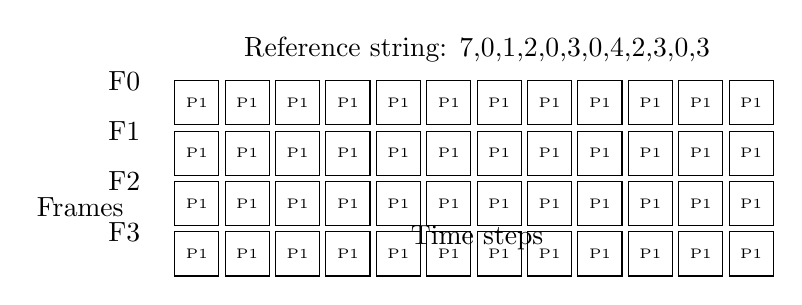
\begin{tikzpicture}[scale=0.8]
  % Draw grid
  \foreach \i in {0,...,3} {
    \node at (-0.8, -\i*0.8) {F\i};
    \foreach \j in {0,...,11} {
      \draw (\j*0.8, -\i*0.8) rectangle ++(0.7, -0.7);
      % Fill với các page ID (placeholder)
      \node[font=\tiny] at (\j*0.8+0.35, -\i*0.8-0.35) {P1};
    }
  }
  
  % Label
  \node at (4.8, 0.5) {Reference string: 7,0,1,2,0,3,0,4,2,3,0,3};
  \node at (-1.5, -2) {Frames};
  \node at (4.8, -2.5) {Time steps};
\end{tikzpicture}
\caption{Lưới khung trang (Frame Grid) minh hoạ}
\label{fig:frame_grid}
\end{figure}

\clearpage
